% ---------------------------------------------------------------------------
% Section 5: Results. Every number is a macro from tables/numbers.tex, which
% paper/gen_numbers.py reads from data/processed/horizon/*/analysis/.
% ---------------------------------------------------------------------------

\section{Results}
\label{sec:results}

\subsection{The transient}
\label{sec:transient}

Figure~\ref{fig:transient}(a) shows the gap over 300 rounds. On the confirmation
set it starts at $\gapZero$, rises to $\peakGap$ at round \peakRound{} and falls to
$\gapNinetyNine$ $[\gapNinetyNineLo, \gapNinetyNineHi]$ at round 99, positive on
all twenty seeds; the exploratory set peaks at $\peakGapExpl$ and is
$\gapNinetyNineExpl$ $[\gapNinetyNineExplLo, \gapNinetyNineExplHi]$ at round 99.
Every one of the forty seeds then enters the margin and stays inside it, and none
is censored. The entry round has a median of \entryMedianConf{} (range
\entryMinConf{}--\entryMaxConf{}) on the confirmation set and \entryMedianExpl{}
(\entryMinExpl{}--\entryMaxExpl{}) on the exploratory set.

Over rounds 250 to 299 the mean gap is $\tailConf$ $[\tailConfLo, \tailConfHi]$,
positive on \tailConfPos{} of twenty seeds. The two one-sided tests reject at
$t = \tostConfLower$ and $\tostConfUpper$ on 19 degrees of freedom, and the 90\%
interval $[\tostConfLo, \tostConfHi]$ lies inside the margin; the exploratory set
gives $\tailExpl$ $[\tailExplLo, \tailExplHi]$ and the same verdict. The registered
predictions for this experiment all held (Table~\ref{tab:predictions}), including
that seeds 42 to 46 reproduce an earlier 300-round run of the same configuration
to every printed digit.

The other arms bound the gap (Figure~\ref{fig:arms}). The oracle's exposure Gini
settles at $\giniOracleTail$ within \oracleSettle{} rounds, as thresholds relax,
and does not move after that: this is the concentration preferences produce. The
NCF arm's Gini falls from the popularity closed form, $1 - 2k/N = 0.96$, to the
oracle's level. At round 0 the oracle, random and popularity arms coincide, because the gate
admits fewer than $k$ candidates and every arm hands out all of them. From round 1
the popularity arm sits at 0.96, and the random arm falls to $\giniRandomTail$.
The peak gap is therefore nearly a closed form: the ranker's $1 - 2k/N = 0.96$
minus the oracle's settled $\giniOracleTail$, about 0.313. What the experiments
measure is how long the ranker takes to leave the common list, not the size of the
peak.

\emph{Exposure converges; welfare does not.} At round 299 the ranker's
algorithmic loss is $\algLossNcfFinal$, against $\algLossOracleFinal$ for the
oracle, a paired difference of $\algLossDiff$ $[\algLossDiffLo, \algLossDiffHi]$
over twenty seeds. The ranker's shortlists agree with the oracle's as sets (mean Jaccard
overlap $\jaccardFinal$) while its scores over the whole other side have a rank
correlation of only $\spearmanFinal$ with true utility. Exposure counts whether an
agent is on a list and not where, and deferred acceptance reads the order, so the
remaining welfare difference is consistent with lists that hold the right agents
in a different order. Within-list order was not measured directly.

\begin{figure}[t]
\centering
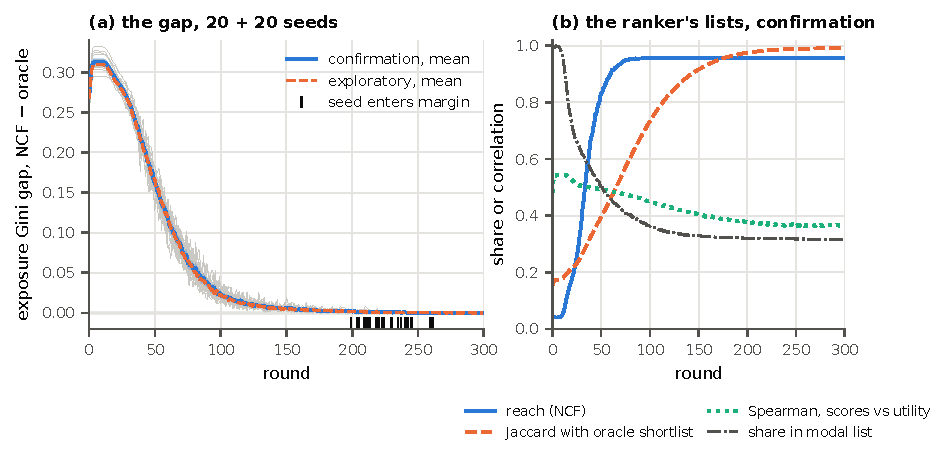
\includegraphics[width=\linewidth]{figures/transient}
\caption{(a) The gap, NCF minus oracle exposure Gini on the same seed and round:
the confirmation-set mean (20 seeds, 95\% $t$ band), the exploratory-set mean (20
seeds), each confirmation seed (thin gray), and each confirmation seed's entry
round (ticks). The shaded strip is the $\pm 0.002$ margin. (b) Diagnostics of the
ranker on the confirmation set: reach; mean Jaccard overlap of an agent's
shortlist with the oracle's; mean Spearman correlation between an agent's scores
and its true utilities over the whole other side; mean share of an agent's
shortlist inside its side's modal list. Source:
\texttt{data/processed/horizon/e09\_canonical/}.}
\label{fig:transient}
\end{figure}

\begin{figure}[t]
\centering
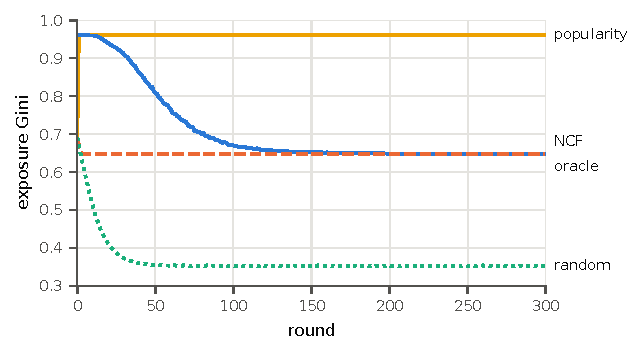
\includegraphics[width=0.62\linewidth]{figures/arms}
\caption{Exposure Gini of the four arms over 300 rounds, mean over the twenty
confirmation seeds. Source: \texttt{data/processed/horizon/e09\_canonical/}.}
\label{fig:arms}
\end{figure}

\subsection{A floor, or a slow decay?}
\label{sec:floor}

A tail inside the margin at round 300 is also what a slow decay would look like
at that horizon, so ten confirmation seeds were run to round 999. Their first 300
rounds reproduce the R2-E9 runs exactly. Three forms were fitted to the seed-mean
gap from its peak to round 500 and judged by how well they predict rounds 501 to
999, which they did not see (Figure~\ref{fig:decay}). The pure exponential
predicts best, with a root-mean-square error of $\rmseExp$ against $\rmseExpConst$
for an exponential to a constant and $\rmsePower$ for a power law. Its half-life is
\halfLife{} rounds, 95\% interval \halfLifeLo{}--\halfLifeHi{} from 2000 resamples
of the seeds. The power law is not a candidate: it predicts a gap of
$\powerAtEnd$ at round 999, several times the margin. The exponential to a
constant fits the first 500 rounds
better by AIC and BIC, but its constant is $\fitK$ $[\fitKLo, \fitKHi]$, a floor
below zero that the held-out rounds contradict.

Over rounds 950 to 999 the gap is $\longTail$ $[\longTailLo, \longTailHi]$,
positive on \longTailPos{} of ten seeds, and the 90\% interval
$[\longTostLo, \longTostHi]$ lies inside the margin. Its change between rounds 900
to 949 and 950 to 999 is $\lateDiff$ $[\lateDiffLo, \lateDiffHi]$, so the series
has stopped moving. By the registered definition this is not a positive floor,
which needed the tail interval to lie above $+0.002$. It is a residual of
\longTailMarginShare{} percent of the margin, inside the range the margin declares
of no consequence, and above zero at ten seeds. The oracle's Gini is constant to every
printed digit from round 300 on, so the residual is a small rise in the ranker's
concentration late in training. Nothing below depends on whether it is real.

\begin{figure}[t]
\centering
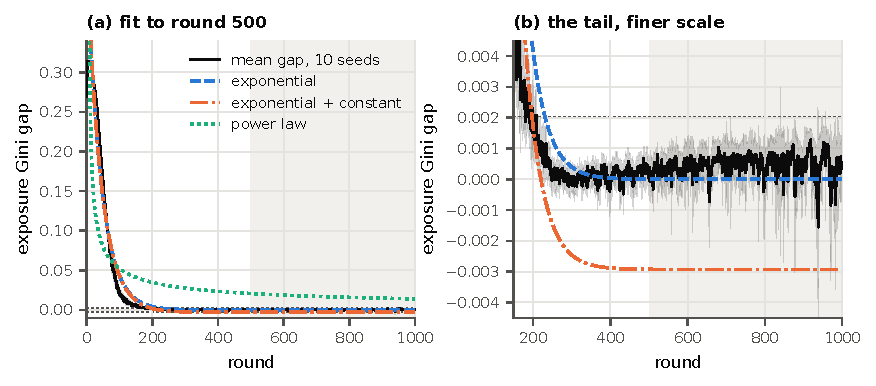
\includegraphics[width=\linewidth]{figures/decay}
\caption{The gap over 1000 rounds, ten confirmation seeds (mean, 95\% $t$ band),
with three forms fitted from the peak to round 500 and evaluated on rounds 501 to
999 (shaded). Dotted lines: the $\pm 0.002$ margin. (b) is the tail of (a) at a
finer scale. Source: \texttt{data/processed/horizon/e10\_long/}.}
\label{fig:decay}
\end{figure}

\subsection{Where it holds}
\label{sec:where}

\paragraph{One knob at a time.} Eight cells each move one modeling knob from its
shipped value: taste spread $\sigma_\tau$ to 0.2 and 1.0, chemistry noise
$\sigma_L$ to 0.5 and 3.0, the weight ratio $\beta/\alpha$ to 1 and 3, and the
status margin $\delta$ to 0 and 1, with ten seeds each over 300 rounds. The
shipped cell is seeds 100 to 109 of the canonical run
(Figure~\ref{fig:sweep}, Table~\ref{tab:sweep}). The five claims were
re-registered as trajectory claims before the cells ran.

The peak gap is positive with an interval excluding zero in all nine cells
(C1t), and its size ranges from $\peakMinCell$ at chemistry noise 0.5 to
$\peakMaxCell$ at 3.0. Near the peak the ranker is still close to the popularity
closed form, so the peak gap is mostly the distance from 0.96 down to the oracle's
Gini, and that distance grows as chemistry noise makes preferences less common:
the oracle's Gini at round 299 is $\oracleGiniShockLow$ at noise 0.5 and
$\oracleGiniShockHigh$ at 3.0. The tail passes the equivalence test in seven of
nine cells (C2t). It fails at chemistry noise 3.0, where the peak is largest and
the tail is $\tailShockHigh$, with \censoredShockHigh{} of ten seeds still outside
the margin at round 299 and a 90\% interval reaching $\tostShockHighHi$; and at
chemistry noise 0.5 for the opposite reason: the
tail is $\tailShockLow$, negative with an interval excluding zero (C5t), and the
ranker ends less concentrated than the oracle. The weight ratio $\beta/\alpha = 3$
also ends with a negative tail, $\tailBetaHigh$, inside the margin; the
registration had predicted a reversal at chemistry noise 0.5 only. Reach at round
299 is at least 0.75 in eight cells (C3t) and $\reachShockLow$ at chemistry noise
0.5, where the oracle's reach is $\reachOracleShockLow$: with little idiosyncratic
taste many agents are on no one's true top twenty. Clearing is non-degenerate
in every cell (C4t). The transient occurs in every cell; its size and length are
set by how common preferences are.

\paragraph{Population size.} At $N = 500$ and $N = 2000$ the shortlist stays at
$k = 20$ and the gate target is set to $\phi = 20/N$, so every agent again starts
with ten admissible candidates and the gate binds; ten seeds each
(Table~\ref{tab:units}). The round-0 Gini is the closed form at each size. The
peak gap is $\peakNFive$, $\peakNTen$ and $\peakNTwenty$ at $N = 500$, 1000 and
2000, falling slightly where the registration predicted a rise. The first round
from which the gap stays below 0.05, $T_{0.05}$, has a mean of \TfiveNFive{},
\TfiveNTen{} and \TfiveNTwenty{} rounds, and at $N = 2000$ \censoredNTwenty{} of
ten seeds are still outside the margin at round 299. The transient is longest in
the largest market, and it is not monotone in $N$.

\paragraph{The horizon in data units.} A length in rounds is a unit of the model.
Every agent's log holds about \rowsPerRound{} rows per round at every $N$, at most
twenty of them positives, so a length in observations per agent is proportional to
a length in rounds and gives the same ratios across $N$. In optimizer steps
$T_{0.05}$ is \stepsTfiveNFive{}, \stepsTfiveNTen{} and \stepsTfiveNTwenty{} at the
three sizes, because a pass over a larger market takes more steps. Neither unit
makes the length independent of market size, so a transient length measured here
does not transfer to another market in rounds, in data or in steps.
Table~\ref{tab:units} gives $T_{0.05}$ in all three units for every experiment
that has one.

\begin{figure}[t]
\centering
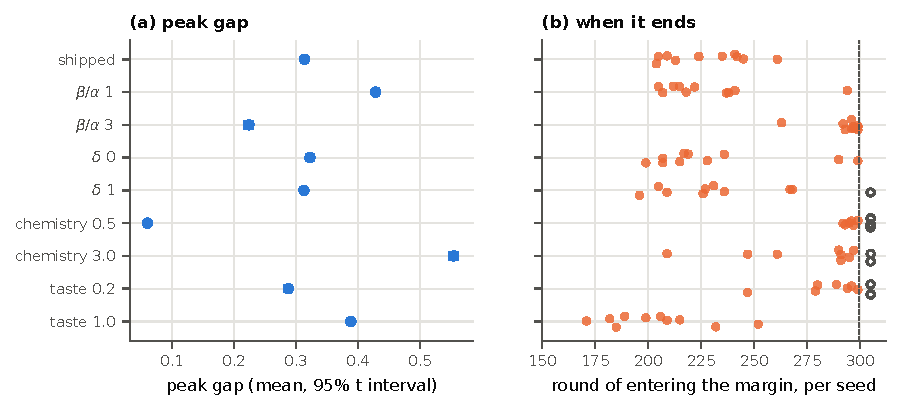
\includegraphics[width=\linewidth]{figures/sweep}
\caption{The one-knob sweep, ten seeds per cell. (a) Peak gap, mean with 95\% $t$
interval. (b) Each seed's entry round; open markers at the right edge are seeds
still outside the margin at round 299. Source:
\texttt{data/processed/horizon/e11\_sweep/} and, for the shipped cell, seeds
100--109 of \texttt{e09\_canonical/}.}
\label{fig:sweep}
\end{figure}

\begin{table}[t]
\centering
\small
\begin{tabular}{lrrrrccccc}
\hline
Cell & Peak gap & Entry & Censored & Tail $\times 10^3$ & C1t & C2t & C3t & C4t & C5t \\
\hline
shipped & 0.314 & 230 & 0 & +0.12 & yes & yes & yes & yes & no \\
$\sigma_\tau = 0.2$ & 0.288 & 295 & 3 & -0.15 & yes & yes & yes & yes & no \\
$\sigma_\tau = 1.0$ & 0.388 & 202 & 0 & -0.12 & yes & yes & yes & yes & no \\
$\sigma_L = 0.5$ & 0.060 & 298 & 4 & -1.85 & yes & \textbf{no} & \textbf{no} & yes & yes \\
$\sigma_L = 3.0$ & 0.554 & 291 & 2 & +1.95 & yes & \textbf{no} & yes & yes & no \\
$\beta/\alpha = 1$ & 0.428 & 220 & 0 & +0.07 & yes & yes & yes & yes & no \\
$\beta/\alpha = 3$ & 0.224 & 296 & 0 & -0.91 & yes & yes & yes & yes & yes \\
$\delta = 0$ & 0.322 & 218 & 0 & -0.15 & yes & yes & yes & yes & no \\
$\delta = 1$ & 0.313 & 229 & 1 & +0.17 & yes & yes & yes & yes & no \\
\hline
\end{tabular}

\caption{The sweep's five trajectory claims, registered before the cells ran.
C1t: peak gap positive, $t$ interval excluding zero. C2t: two one-sided tests on
the rounds 250--299 tail pass at $\pm 0.002$. C3t: reach at round 299 at least
0.75. C4t: clearing rate at round 299 with an interval excluding zero. C5t: tail
mean negative with an interval excluding zero (a reversal). Ten seeds per cell.
Source: \texttt{data/processed/horizon/e11\_sweep/analysis/cells.csv}.}
\label{tab:sweep}
\end{table}

\begin{table}[t]
\centering
\footnotesize
\begin{tabular}{llrrrr}
\hline
Experiment & Condition & Rounds & Rows per agent & Optimizer steps & Censored \\
\hline
R2-E9 & shipped, confirmation & 87 & 8{,}512 & 2{,}131 & 0 of 20 \\
R2-E9 & shipped, exploratory & 86 & 8{,}395 & 2{,}102 & 0 of 20 \\
R2-E11 & $\beta/\alpha = 1$ & 93 & 9{,}142 & 2{,}287 & 0 of 10 \\
R2-E11 & $\beta/\alpha = 3$ & 81 & 7{,}849 & 1{,}968 & 0 of 10 \\
R2-E11 & $\delta = 0$ & 85 & 8{,}338 & 2{,}088 & 0 of 10 \\
R2-E11 & $\delta = 1$ & 88 & 8{,}615 & 2{,}158 & 0 of 10 \\
R2-E11 & $\sigma_L = 0.5$ & 26 & 2{,}458 & 618 & 0 of 10 \\
R2-E11 & $\sigma_L = 3.0$ & 113 & 11{,}204 & 2{,}803 & 0 of 10 \\
R2-E11 & $\sigma_\tau = 0.2$ & 85 & 8{,}278 & 2{,}075 & 0 of 10 \\
R2-E11 & $\sigma_\tau = 1.0$ & 87 & 8{,}539 & 2{,}136 & 0 of 10 \\
R2-E13a & 0.5 passes per round & 174 & 17{,}067 & 2{,}190 & 0 of 10 \\
R2-E13a & 2 passes per round & 44 & 4{,}260 & 2{,}133 & 0 of 10 \\
R2-E13a & 4 passes per round & 22 & 2{,}142 & 2{,}144 & 0 of 10 \\
R2-E13c & off-policy, oracle market's data & 75 & not logged & 1{,}865 & 0 of 10 \\
R2-E13c & off-policy, random market's data & 75 & not logged & 1{,}878 & 0 of 10 \\
R2-E13d & warm start, confirmation & 62 & 6{,}146 & 2{,}642 & 0 of 20 \\
R2-E13d & warm start, exploratory & 63 & 6{,}210 & 2{,}659 & 0 of 20 \\
R2-E17 & N = 500 & 95 & 9{,}296 & 1{,}188 & 0 of 10 \\
R2-E17 & N = 2000 & 136 & 13{,}377 & 6{,}580 & 0 of 10 \\
\hline
\end{tabular}

\caption{$T_{0.05}$, the first round from which the gap stays below 0.05, in
three units: rounds, rows of training log per agent, and optimizer steps. Mean
over seeds; censored seeds are excluded and counted. Sources:
\texttt{data/processed/horizon/} (\texttt{e09\_canonical}, \texttt{e11\_sweep},
\texttt{e13a\_dose}, \texttt{e13c\_offpolicy}, \texttt{e13d\_warm},
\texttt{e17\_size}).}
\label{tab:units}
\end{table}

\subsection{What ends it}
\label{sec:what-ends}

\paragraph{The common list breaks up.} At round 0 a per-candidate term explains at
least $\itemShareZeroMin$ of the within-agent variation in the untrained ranker's
scores on every one of the forty seeds, at least $\modalShareZeroMin$ of every
agent's shortlist is its side's modal list, and the exposure Gini is within
$\giniZeroMaxDev$ of the popularity closed form (Figure~\ref{fig:transient}(b)).
Every agent on a side sees nearly the same twenty candidates. As training proceeds
the share of identical lists falls below 0.1 by round \identicalBelowRound{}, the
per-candidate term's share of score variation falls below one half by round
\itemBelowRound{}, and the mean overlap of an agent's shortlist with the oracle's
rises from $\jaccardZero$ to $\jaccardFinal$.

The registered prediction tied the gap to ranking quality measured as the rank
correlation between an agent's scores and its utilities over the whole other
side. It failed in sign: across rounds 6 to 299 the gap and that correlation are
positively correlated on every seed (median $\corrMedian$, minimum $\corrMin$),
because the correlation falls as the gap closes. The ranker starts by ordering
every agent's candidates by one shared score, which agrees moderately with each
agent's own utility because the candidates many agents value share high status
and attractiveness. It then learns which twenty candidates each agent ranks
highest, and its training labels separate those twenty from uniform negatives
without ordering the rest. The gap is a quantity about the top twenty, and among
these diagnostics it is the overlap with the oracle's shortlist and the breakup of
the modal list that move with it.

\paragraph{Optimizer steps, not rounds.} Training at 0.5, 1, 2 and 4 passes per
round, ten seeds each, the gap stays below 0.05 from round \TfiveDoseHalf{},
\TfiveDoseOne{}, \TfiveDoseTwo{} and \TfiveDoseFour{} on average: doubling the
passes halves the length (Figure~\ref{fig:dose}(a)). In cumulative optimizer
steps the four curves fall on one (Figure~\ref{fig:dose}(b)), and the step count
at that threshold is between \stepsTfiveMin{} and \stepsTfiveMax{} at every dose.
The elasticity of the length in rounds with respect to the dose is
$\doseElasticity$ $[\doseElasticityLo, \doseElasticityHi]$, as registered. Each
round's log draws on nearly the same distribution as the last, so what the
transient takes is optimizer steps. At four passes the gap overshoots: it ends at
$\doseFourTail$, below the margin, with \doseFourCensored{} of ten seeds outside
it at round 299. More training eventually leaves this ranker less concentrated
than the oracle, and this experiment does not say why.

\paragraph{Feedback through thresholds.} A second ranker, trained each round on
the log of a market it does not control (one run by the oracle rule or by the
random rule), starts from the same weights and, at round 0, the same data as the
market's own ranker; the thresholds are what differ after that. At round 49 its gap
is smaller than the market ranker's by $\offOracleFortyNine$ $[\offOracleFortyNineLo,
\offOracleFortyNineHi]$ on the oracle market's data and by $\offRandomFortyNine$
$[\offRandomFortyNineLo, \offRandomFortyNineHi]$ on the random market's
(Figure~\ref{fig:feedback}(a)). The registered prediction, a difference under
0.01, failed. The effect is about \offShare{} percent of the gap at that round,
about \offDelay{} rounds of decay at that point of the curve, and it is gone by
round 299. The mechanism is the one channel of \S\ref{sec:log}: concentrated shortlists
leave many acceptors without proposals, their thresholds stay high, and their
logged positives stay truncated for longer. Feedback delays the end of the
transient; it does not sustain it.

\paragraph{Exploration.} Replacing the last $m$ entries of every shortlist with
candidates drawn uniformly ($m = 1$ or $4$ of 20) lowers the whole-list gap by
construction. The quantity of interest is the gap of the exploiting part, the
first $20 - m$ entries against the oracle's first $20 - m$. Its difference from
the non-exploring ranker's gap is $\expOneFortyNine$ at round 49 and
$\expOneNinetyNine$ at round 99 at $m = 1$, and $\expFourFortyNine$ and
$\expFourNinetyNine$ at $m = 4$; every interval excludes zero except the one at
round 49 for $m = 4$, and the registered prediction of a difference inside $\pm
0.01$ fails (Figure~\ref{fig:feedback}(b)). The likely route is the same: random
slots spread proposals and so relax more thresholds. At round 299 the exploiting
part ends above the control, $\expOneTwoNinetyNine$ at $m = 1$. Cutting a list
by utility rank and by score rank differs even when the two lists hold the same
agents, so a check added after these results were read compares the exploring
ranker's head with a non-exploring ranker's head of the same length. On that
comparison the round-299 excess is $\checkExploitTwoNinetyNine$
$[\checkExploitTwoNinetyNineLo, \checkExploitTwoNinetyNineHi]$, an interval that
includes zero, so the late excess was the comparator's; the faster closing is not:
the differences at rounds 49 and 99 are $\checkOneFortyNine$ and
$\checkOneNinetyNine$ at $m = 1$ and $\checkFourFortyNine$ and
$\checkFourNinetyNine$ at $m = 4$, every interval excluding zero.

\paragraph{An informed start.} Pretraining the ranker for fifty passes on the
round-0 log before the market opens raises round-0 reach from $\reachZeroControl$
to $\reachZeroWarm$ and cuts the round-0 gap from $\gapZeroControl$ to
$\gapZeroWarm$ (forty seeds). On the registered measure, the warm arm's fall from
round 0 to round 299 as a share of the control's, $\warmShareConf$ percent
$[\warmShareConfLo, \warmShareConfHi]$ of the decay survives on the confirmation
set and $\warmShareExpl$ percent on the exploratory set: the informed start removes
about four fifths of it (Table~\ref{tab:warm}). The registered upper bound of
one half held; the registered round-0 reach above 0.8 held on every seed but one
($\reachWarmMin$). The share is larger on levels, because the oracle's Gini also
falls in both arms, and near 0.7 measured from each arm's own peak, because the
warm arm climbs for a few rounds from its informed start before it decays. By
round 299 the two arms differ by $\warmTerminalTwoNinetyNine$ on the confirmation
set. Fifty passes over one log add optimizer steps without adding data, and they
are not worth as much as steps on fresh logs: the warm arm's gap stays below 0.05
from round \TfiveWarm{} against \TfiveControl{} for the control, sooner in rounds,
but after \stepsTfiveWarm{} optimizer steps against \stepsTfiveControl{}
(Table~\ref{tab:units}). The dose result's steps are steps on a new log each
round.

\begin{figure}[t]
\centering
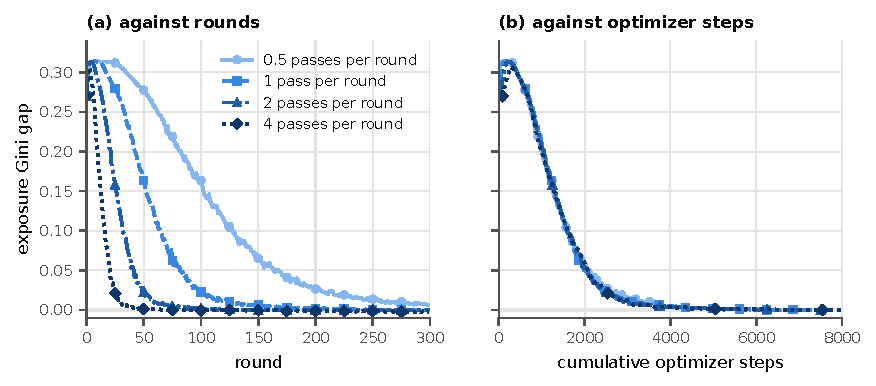
\includegraphics[width=\linewidth]{figures/dose}
\caption{The gap at four training doses, ten seeds each (mean), against rounds (a)
and against cumulative optimizer steps (b). Shaded strip: the $\pm 0.002$ margin.
Source: \texttt{data/processed/horizon/e13a\_dose/} and, for one pass, seeds
100--109 of \texttt{e09\_canonical/}.}
\label{fig:dose}
\end{figure}

\begin{figure}[t]
\centering
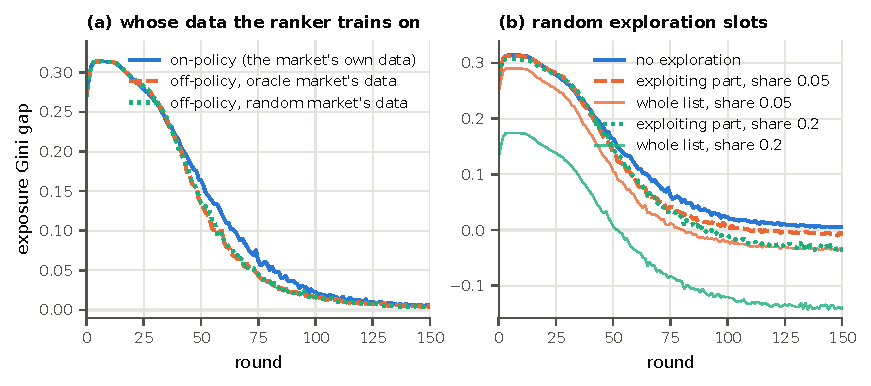
\includegraphics[width=\linewidth]{figures/feedback}
\caption{(a) The gap of a ranker trained on its own market's data (on-policy)
and of a ranker trained on the data of a market run by the oracle or the random
rule (off-policy), ten seeds, mean. (b) With exploration slots: the gap of the
exploiting part of each list and of the whole list, against the non-exploring
ranker, ten seeds, mean. Source: \texttt{data/processed/horizon/e13c\_offpolicy/},
\texttt{e13b\_explore/}, \texttt{e09\_canonical/}.}
\label{fig:feedback}
\end{figure}

\begin{table}[t]
\centering
\small
\begin{tabular}{llrr}
\hline
Quantity & Basis & Confirmation (100--119) & Exploratory (42--61) \\
\hline
gap (primary) & round 0 & 20.8\% [17.9, 23.6] & 24.0\% [21.9, 26.1] \\
level & round 0 & 32.0\% [29.4, 34.6] & 34.4\% [32.7, 36.1] \\
gap & own peak & 69.1\% [67.8, 70.4] & 68.3\% [67.1, 69.4] \\
level & own peak & 69.3\% [68.0, 70.6] & 68.6\% [67.4, 69.8] \\
\hline
\end{tabular}

\caption{Share of the control arm's decay that survives a warm start, four
constructions, each computed per seed and averaged, 95\% $t$ interval over twenty
seeds per set. Round-0 basis: (warm$_0$ $-$ warm$_{299}$) / (control$_0$ $-$
control$_{299}$); peak basis: each arm from its own maximum. Gap: NCF minus oracle
Gini; level: NCF Gini. The registered primary is the gap on the round-0 basis.
Source: \texttt{data/processed/horizon/e13d\_warm/analysis/summary.csv}.}
\label{tab:warm}
\end{table}

\subsection{An open market}
\label{sec:arrivals}

In every run so far the population is fixed, so the ranker eventually learns every
agent. When a share $\nu$ of the slots is replaced every round by fresh agents
with new traits, new embeddings and calibrated thresholds (\S\ref{sec:open}),
some agents are always new. Over rounds 500 to 599 the gap is $\openGapLow$
$[\openGapLowLo, \openGapLowHi]$ at $\nu = 0.5$ percent per round, $\openGapMid$
$[\openGapMidLo, \openGapMidHi]$ at 1 percent and $\openGapHigh$
$[\openGapHighLo, \openGapHighHi]$ at 2 percent, positive on every seed and
increasing in the rate, as registered (Figure~\ref{fig:arrivals}(a), ten seeds per
rate). At every rate it is above the margin.

The registered stationarity check fails at every rate. Its paired comparison of
rounds 590--599 with 580--589 finds no change ($p = \statPLow$, $\statPMid$ and
$\statPHigh$), but its second criterion, a largest round-to-round step in the
seed-mean series below a tenth of the seed standard deviation, fails: the step is
\stepRatioLow{}, \stepRatioMid{} and \stepRatioHigh{} of it. That criterion was
written for the closed market, whose series stops moving; here every round's
arrivals move every round's mean. A trend test added after this was read finds the
gap still moving over rounds 400 to 599: it changes by $\trendLow$ $[\trendLowLo,
\trendLowHi]$ at 0.5 percent per round, $\trendMid$ $[\trendMidLo, \trendMidHi]$
at 1 percent and $\trendHigh$ $[\trendHighLo, \trendHighHi]$ at 2 percent, every
interval excluding zero. At the lowest rate the gap is still falling, so its level
over rounds 500 to 599 overstates the gap at the end of the run; at the two higher
rates it is rising. None of the three levels is a steady state at 600 rounds.
What survives is the weaker statement the trend allows: at every rate the
gap stays above the margin to the end of the run, and it is larger at a higher
rate.

By tenure (Figure~\ref{fig:arrivals}(b)), agents in their first ten rounds receive
a share of the ranker's exposure below their share of the population at 1 and 2
percent per round ($\cohortNewMid$ and $\cohortNewHigh$ of proportional), while the
oracle gives them close to their share ($\cohortNewMidOracle$ and
$\cohortNewHighOracle$), and agents with fifty rounds or more receive more than
their share ($\cohortOldLow$, $\cohortOldMid$, $\cohortOldHigh$). At 0.5 percent
per round the newest agents are over-exposed instead ($\cohortNewLow$), which
fails the registered prediction that they are under-exposed at every rate.

The ordering follows from a ratio. An agent stays for $1/\nu$ rounds on average,
200, 100 and 50 rounds at the three rates, against a closed-market entry round of
about \entryMedianConf{}, so a higher rate leaves a larger share of agents newer than
the ranker's learning time. No rate with $1/\nu$ well above that time was run, so
the experiment shows that the gap tracks this ratio and does not locate where it
falls inside the margin.

A round has no calendar length here, so a replacement rate per round cannot be
read as a platform's churn without knowing how many rounds of retraining a
platform's period contains. What the open market shows is that the gap tracks the
rate at which the ranker meets agents it has not learned, and that it stays above
the margin at every rate tested.

\begin{figure}[t]
\centering
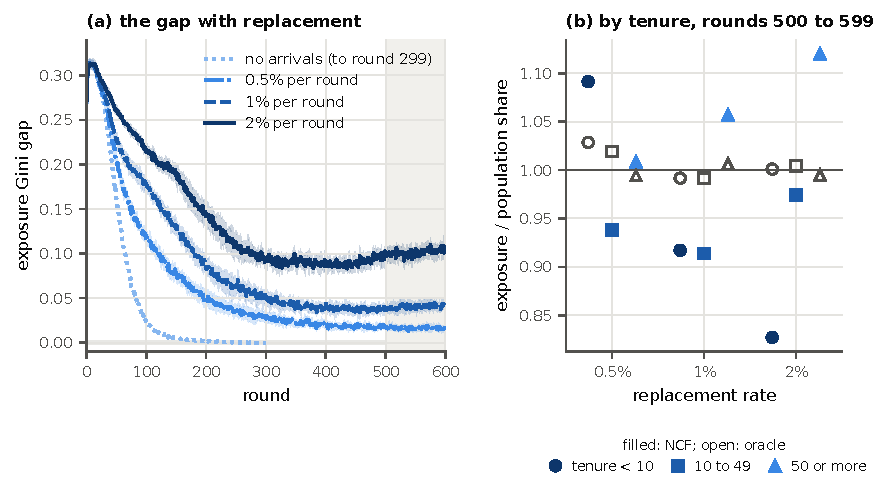
\includegraphics[width=\linewidth]{figures/arrivals}
\caption{(a) The gap with a share of agents replaced each round, ten seeds per
rate (mean, 95\% $t$ band), and the closed market (seeds 100--119, to round 299).
Shaded: rounds 500 to 599, over which the levels are read. (b) Each tenure band's
share of exposure divided by its share of agents, rounds 500 to 599: NCF (filled)
and oracle (open). Source: \texttt{data/processed/horizon/e14\_arrivals/}.}
\label{fig:arrivals}
\end{figure}
